\documentclass[tikz,border=5pt]{standalone}
\usepackage[UTF8]{ctex}\usepackage{amsmath,amssymb}
\usetikzlibrary{arrows.meta,calc}
\definecolor{ink}{HTML}{243447}\definecolor{blue}{HTML}{2765A2}
\definecolor{green}{HTML}{3F7D5B}\definecolor{red}{HTML}{B74739}
\tikzset{body/.style={draw=ink,thick},vec/.style={draw=blue,thick,-{Latex}},guide/.style={gray!65,dashed},dim/.style={ink,{Latex}-{Latex}},line cap=round,line join=round}
\begin{document}
\begin{tikzpicture}
 \draw[body](0,0)circle(1.65);
 \draw[vec](-2.2,0)--(2.3,0)node[right]{$x$};
 \draw[vec](0,-2.1)--(0,2.2)node[above]{$y$};
 \fill[red](0,1.65)circle(.055);
 \draw[red,thick,-{Latex}](0,1.65)--(1.3,1.65)node[midway,above]{$v_0$};
 \node[above left]at(0,1.65){$m,q$};
 \foreach\p in{(-1.9,1.8),(1.9,1.1),(-1.9,-1.4),(1.9,-1.4)}
 {\node[blue]at\p{$\otimes$};}
 \node[blue]at(2.45,1.85){$B_0$向内};
 \draw[dim](-.08,-.08)--(-1.17,-1.17)node[midway,below right]{$r$};
\end{tikzpicture}
\begin{tikzpicture}
 \draw[body](0,0)circle(1.65);
 \node[blue]at(0,0){$\otimes\,\dot B>0$};
 \draw[green,thick,-{Latex}](1.85,0)arc[start angle=0,end angle=110,radius=1.85];
 \node[green,above]at(.65,1.85){$\boldsymbol E$};
 \fill[red](0,1.65)circle(.045);
 \draw[red,thick,-{Latex}](0,1.65)--(1.1,1.65)node[midway,below]{$w>0$};
 \draw[green,thick,-{Latex}](0,1.65)--(-1.1,1.65);
 \node at(0,-2.25){顺时针为正：$E_\parallel=-\tfrac r2\dot B$};
\end{tikzpicture}
\begin{tikzpicture}[x={(1cm,0cm)},y={(.35cm,.25cm)},z={(0cm,1cm)}]
 \draw[guide,domain=0:360,samples=81]plot({1.65*cos(\x)},{1.65*sin(\x)},0);
 \draw[blue,dashed,thick,domain=180:360,samples=61]plot({1.65*cos(\x)},{1.65*sin(\x)*cos(50)},{1.65*sin(\x)*sin(50)});
 \draw[blue,thick,domain=0:180,samples=61]plot({1.65*cos(\x)},{1.65*sin(\x)*cos(50)},{1.65*sin(\x)*sin(50)});
 \draw[vec](-2.3,0,0)--(2.5,0,0)node[right]{$x$固定};
 \draw[green,thick,-{Latex}](0,0,0)--(0,{1.65*sin(50)},{-1.65*cos(50)})node[below right]{$\boldsymbol n_{\rm cw}$};
 \draw[vec](3,1,2.1)--(3,1,.45)node[midway,right]{$\boldsymbol B=-B_0\boldsymbol e_z$};
 \fill[red](0,{1.65*cos(50)},{1.65*sin(50)})circle(.045);
 \node[above]at(0,{1.65*cos(50)},{1.65*sin(50)}){$P$};
 \draw[red,thick,-{Latex}](0,{1.65*cos(50)},{1.65*sin(50)})--(1,{1.65*cos(50)},{1.65*sin(50)})node[midway,above]{$w$};
 \node at(0,0,-2){灰色为初始环面；蓝色为转动后的环面};
 \node at(0,0,-2.5){$\Phi_B=\pi r^2B_0\cos\lambda$（顺时针法向）};
\end{tikzpicture}
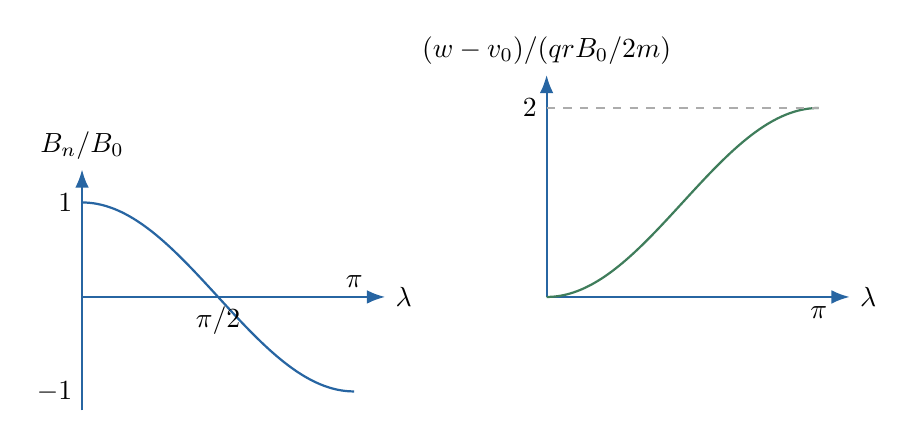
\begin{tikzpicture}
 \begin{scope}[x=1.1cm,y=1.2cm]
 \draw[vec](0,0)--(3.5,0)node[right]{$\lambda$};
 \draw[vec](0,-1.2)--(0,1.35)node[above]{$B_n/B_0$};
 \draw[blue,thick,domain=0:pi,samples=91]plot(\x,{cos(\x r)});
 \node[left]at(0,1){$1$};\node[left]at(0,-1){$-1$};
 \node[below]at(1.5708,0){$\pi/2$};\node[above]at(3.1416,0){$\pi$};
 \end{scope}
 \begin{scope}[shift={(5.9,0)},x=1.1cm,y=1.2cm]
 \draw[vec](0,0)--(3.5,0)node[right]{$\lambda$};
 \draw[vec](0,0)--(0,2.35)node[above]{$(w-v_0)/(qrB_0/2m)$};
 \draw[green,thick,domain=0:pi,samples=91]plot(\x,{1-cos(\x r)});
 \draw[guide](0,2)--(3.1416,2);
 \node[left]at(0,2){$2$};\node[below]at(3.1416,0){$\pi$};
 \end{scope}
\end{tikzpicture}
\end{document}
